\documentclass{standalone}
\usepackage{tikz}
\usetikzlibrary{patterns}
\usetikzlibrary{positioning}
\usetikzlibrary{patterns, positioning}
\usetikzlibrary{shapes.misc}
\usepackage[outline]{contour}
\contourlength{1.5pt} 
\usepackage[sfdefault]{ClearSans}

\begin{document}
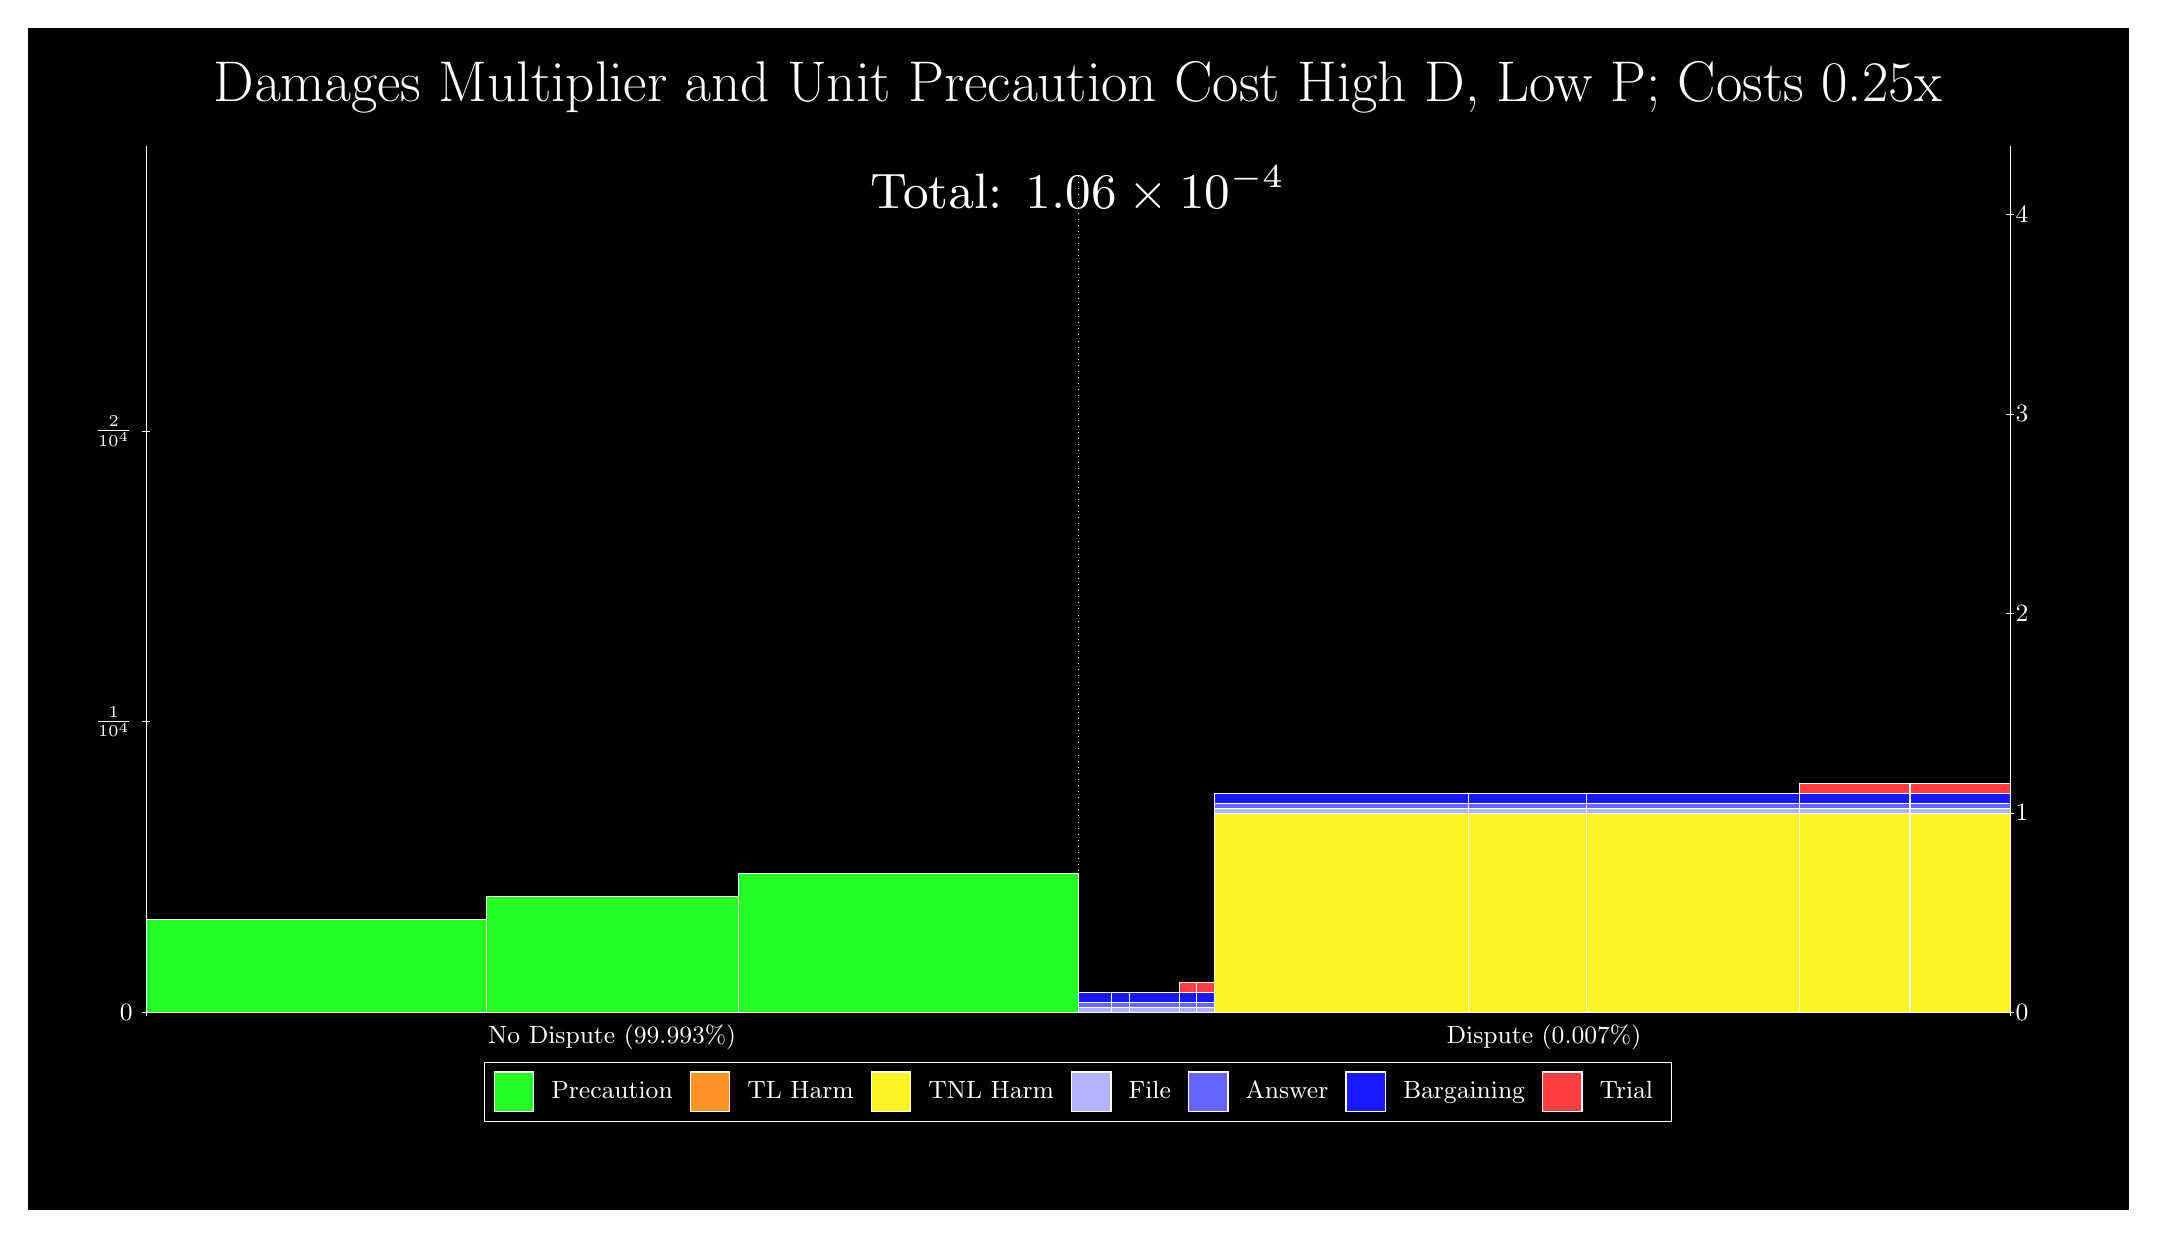
\begin{tikzpicture}
\draw[fill=black] (0,0) rectangle (26.667,15);
\draw[draw=none,text=white] (0,13.5) rectangle (26.667,15) node[midway] {\huge Damages Multiplier and Unit Precaution Cost High D, Low P; Costs 0.25x};
\draw[fill=green!85,draw=white,very thin] (1.5,2.5) rectangle (5.8206,3.6814);
\draw[fill=green!85,draw=white,very thin] (5.8206,2.5) rectangle (9.0126,3.9768);
\draw[fill=green!85,draw=white,very thin] (9.0126,2.5) rectangle (13.333,4.2722);
\draw[fill=green!85,draw=white,very thin] (13.333,2.5) rectangle (13.755,2.5001);
\draw[fill=blue!30,draw=white,very thin] (13.333,2.5001) rectangle (13.755,2.5634);
\draw[fill=blue!60,draw=white,very thin] (13.333,2.5634) rectangle (13.755,2.6268);
\draw[fill=blue!90,draw=white,very thin] (13.333,2.6268) rectangle (13.755,2.7535);
\draw[fill=green!85,draw=white,very thin] (13.755,2.5) rectangle (13.987,2.5001);
\draw[fill=blue!30,draw=white,very thin] (13.755,2.5001) rectangle (13.987,2.5635);
\draw[fill=blue!60,draw=white,very thin] (13.755,2.5635) rectangle (13.987,2.6268);
\draw[fill=blue!90,draw=white,very thin] (13.755,2.6268) rectangle (13.987,2.7535);
\draw[fill=green!85,draw=white,very thin] (13.987,2.5) rectangle (14.624,2.5001);
\draw[fill=blue!30,draw=white,very thin] (13.987,2.5001) rectangle (14.624,2.5635);
\draw[fill=blue!60,draw=white,very thin] (13.987,2.5635) rectangle (14.624,2.6268);
\draw[fill=blue!90,draw=white,very thin] (13.987,2.6268) rectangle (14.624,2.7536);
\draw[fill=green!85,draw=white,very thin] (14.624,2.5) rectangle (14.828,2.5001);
\draw[fill=blue!30,draw=white,very thin] (14.624,2.5001) rectangle (14.828,2.5634);
\draw[fill=blue!60,draw=white,very thin] (14.624,2.5634) rectangle (14.828,2.6268);
\draw[fill=blue!90,draw=white,very thin] (14.624,2.6268) rectangle (14.828,2.7535);
\draw[fill=red!75,draw=white,very thin] (14.624,2.7535) rectangle (14.828,2.8802);
\draw[fill=green!85,draw=white,very thin] (14.828,2.5) rectangle (15.062,2.5001);
\draw[fill=blue!30,draw=white,very thin] (14.828,2.5001) rectangle (15.062,2.5635);
\draw[fill=blue!60,draw=white,very thin] (14.828,2.5635) rectangle (15.062,2.6268);
\draw[fill=blue!90,draw=white,very thin] (14.828,2.6268) rectangle (15.062,2.7535);
\draw[fill=red!75,draw=white,very thin] (14.828,2.7535) rectangle (15.062,2.8803);
\draw[fill=green!85,draw=white,very thin] (15.062,2.5) rectangle (18.291,2.5001);
\draw[fill=yellow!85,draw=white,very thin] (15.062,2.5001) rectangle (18.291,5.0344);
\draw[fill=blue!30,draw=white,very thin] (15.062,5.0344) rectangle (18.291,5.0978);
\draw[fill=blue!60,draw=white,very thin] (15.062,5.0978) rectangle (18.291,5.1612);
\draw[fill=blue!90,draw=white,very thin] (15.062,5.1612) rectangle (18.291,5.2879);
\draw[fill=green!85,draw=white,very thin] (18.291,2.5) rectangle (19.786,2.5001);
\draw[fill=yellow!85,draw=white,very thin] (18.291,2.5001) rectangle (19.786,5.0345);
\draw[fill=blue!30,draw=white,very thin] (18.291,5.0345) rectangle (19.786,5.0978);
\draw[fill=blue!60,draw=white,very thin] (18.291,5.0978) rectangle (19.786,5.1612);
\draw[fill=blue!90,draw=white,very thin] (18.291,5.1612) rectangle (19.786,5.2879);
\draw[fill=green!85,draw=white,very thin] (19.786,2.5) rectangle (22.488,2.5001);
\draw[fill=yellow!85,draw=white,very thin] (19.786,2.5001) rectangle (22.488,5.0345);
\draw[fill=blue!30,draw=white,very thin] (19.786,5.0345) rectangle (22.488,5.0978);
\draw[fill=blue!60,draw=white,very thin] (19.786,5.0978) rectangle (22.488,5.1612);
\draw[fill=blue!90,draw=white,very thin] (19.786,5.1612) rectangle (22.488,5.2879);
\draw[fill=green!85,draw=white,very thin] (22.488,2.5) rectangle (23.887,2.5001);
\draw[fill=yellow!85,draw=white,very thin] (22.488,2.5001) rectangle (23.887,5.0344);
\draw[fill=blue!30,draw=white,very thin] (22.488,5.0344) rectangle (23.887,5.0978);
\draw[fill=blue!60,draw=white,very thin] (22.488,5.0978) rectangle (23.887,5.1612);
\draw[fill=blue!90,draw=white,very thin] (22.488,5.1612) rectangle (23.887,5.2879);
\draw[fill=red!75,draw=white,very thin] (22.488,5.2879) rectangle (23.887,5.4146);
\draw[fill=green!85,draw=white,very thin] (23.887,2.5) rectangle (23.908,2.5001);
\draw[fill=orange!85,draw=white,very thin] (23.887,2.5001) rectangle (23.908,5.0344);
\draw[fill=blue!30,draw=white,very thin] (23.887,5.0344) rectangle (23.908,5.0978);
\draw[fill=blue!60,draw=white,very thin] (23.887,5.0978) rectangle (23.908,5.1612);
\draw[fill=blue!90,draw=white,very thin] (23.887,5.1612) rectangle (23.908,5.2879);
\draw[fill=red!75,draw=white,very thin] (23.887,5.2879) rectangle (23.908,5.4146);
\draw[fill=green!85,draw=white,very thin] (23.908,2.5) rectangle (25.167,2.5001);
\draw[fill=yellow!85,draw=white,very thin] (23.908,2.5001) rectangle (25.167,5.0345);
\draw[fill=blue!30,draw=white,very thin] (23.908,5.0345) rectangle (25.167,5.0978);
\draw[fill=blue!60,draw=white,very thin] (23.908,5.0978) rectangle (25.167,5.1612);
\draw[fill=blue!90,draw=white,very thin] (23.908,5.1612) rectangle (25.167,5.2879);
\draw[fill=red!75,draw=white,very thin] (23.908,5.2879) rectangle (25.167,5.4146);
\node[font=\small,text=white,anchor=north,scale=2] at (13.333, 13.5) {Total: $1.06\times 10^{-4}$};
\draw[white,very thin] (1.5,2.5) -- (1.5,13.5);
\draw[white,very thin] (1.45,2.5) -- (1.55,2.5);
\node[font=\small,text=white, anchor=east] at (1.45, 2.5) {0};
\draw[white,very thin] (1.45,6.192) -- (1.55,6.192);
\node[font=\small,text=white, anchor=east] at (1.45, 6.192) {$\frac{1}{10^{4}}$};
\draw[white,very thin] (1.45,9.884) -- (1.55,9.884);
\node[font=\small,text=white, anchor=east] at (1.45, 9.884) {$\frac{2}{10^{4}}$};

\draw[white,dotted,very thin] (13.333,2.83) -- (13.333,13.17);
\draw[white,very thin] (25.167,2.5) -- (25.167,13.5);
\draw[white,very thin] (25.117,2.5) -- (25.217,2.5);
\node[font=\small,text=white, anchor=west] at (25.117, 2.5) {0};
\draw[white,very thin] (25.117,5.0344) -- (25.217,5.0344);
\node[font=\small,text=white, anchor=west] at (25.117, 5.0344) {1};
\draw[white,very thin] (25.117,7.5687) -- (25.217,7.5687);
\node[font=\small,text=white, anchor=west] at (25.117, 7.5687) {2};
\draw[white,very thin] (25.117,10.103) -- (25.217,10.103);
\node[font=\small,text=white, anchor=west] at (25.117, 10.103) {3};
\draw[white,very thin] (25.117,12.637) -- (25.217,12.637);
\node[font=\small,text=white, anchor=west] at (25.117, 12.637) {4};

\draw[white,very thin] (1.5,2.5) -- (25.167,2.5);
\draw[white,very thin] (1.5,2.45) -- (1.5,2.55);
\node[font=\small,text=white, anchor=north] at (1.5, 2.45) {};
\draw[white,very thin] (25.167,2.45) -- (25.167,2.55);
\node[font=\small,text=white, anchor=north] at (25.167, 2.45) {};

\node[font=\small,text=white,anchor=south] at (7.4167, 1.9) {No\ Dispute\ (99.993\%)};
\node[font=\small,text=white,anchor=south] at (19.25, 1.9) {Dispute\ (0.007\%)};
\draw (13.3333,2.5) node (B) {};
\begin{scope}[align=center]
\matrix[scale=0.5,draw=white,below=0.5cm of B,nodes={draw},column sep=0.1cm]{
\node[rectangle,draw,minimum width=0.5cm,minimum height=0.5cm,fill=green!85]{}; & \node[draw=none,font=\small,text=white]{Precaution}; &
\node[rectangle,draw,minimum width=0.5cm,minimum height=0.5cm,fill=orange!85]{}; & \node[draw=none,font=\small,text=white]{TL Harm}; &
\node[rectangle,draw,minimum width=0.5cm,minimum height=0.5cm,fill=yellow!85]{}; & \node[draw=none,font=\small,text=white]{TNL Harm}; &
\node[rectangle,draw,minimum width=0.5cm,minimum height=0.5cm,fill=blue!30]{}; & \node[draw=none,font=\small,text=white]{File}; &
\node[rectangle,draw,minimum width=0.5cm,minimum height=0.5cm,fill=blue!60]{}; & \node[draw=none,font=\small,text=white]{Answer}; &
\node[rectangle,draw,minimum width=0.5cm,minimum height=0.5cm,fill=blue!90]{}; & \node[draw=none,font=\small,text=white]{Bargaining}; &
\node[rectangle,draw,minimum width=0.5cm,minimum height=0.5cm,fill=red!75]{}; & \node[draw=none,font=\small,text=white]{Trial}; \\\\
};\end{scope}

\end{tikzpicture}
\end{document}